%%% ssid.tex :: mito / nyamcoder %%%
\documentclass{article}
\usepackage{CJKutf8}
\usepackage[dvipsnames]{xcolor}
\usepackage{pst-plot,pst-text}
\newcommand\texthan{\textbf{\textcolor{OrangeRed}{신사임당}(申師任堂, 1504년$\sim$1551
년)} 은 조선 시대의 여류 문인이자 화가이다. 5 만원권의 도안 인물이기도 하다. \textcolor{OrangeRed}
{신사임당} 은 강원도 \textcolor{Emerald}{강릉}  태생으로 그의 생가 \textcolor{Emerald}{오죽헌}
은 지금도 보존되고 있다.\qquad  본명은 \textcolor{OrangeRed}{신인선}이었다.  아버지는 \textcolor
{Emerald}{신명화(申命和)} 라는 이름의 선비였고,  어머니는 \textcolor{Emerald}{ 용인 이씨} 집안의
선비인 이사온의 딸이었다.  스스로 \textcolor{OrangeRed}{사임당(師任堂)} 이라는 호를 지었는데, 주나
라의 기틀을 닦은 문왕의 어머니 \textcolor{RoyalBlue}{태임(太任)} 에서 따왔다고 전한다.  그 외에
\textcolor{RoyalBlue}{인임당(姻姙堂)}  또는 \textcolor{RoyalBlue}{임사제(姙師齊)} 라는 호도 가
졌다고 한다.\qquad 1522 년 덕수 이씨의 \textcolor{Emerald}{이원수(李元秀)} 와 결혼하여 강릉에서
서울로 이사했으며 4 남 3 녀를 두었다. \textcolor{Emerald}{ 율곡 이이} 는 \textcolor{OrangeRed}{신
사임당} 의 셋째 아들이다.  그는 뛰어난 \textcolor{Thistle}{화가} 로서 7 살 때 세종 시대의 화가 안견
의 그림을 본따서 그림을 그렸고, 숙종,  송시열 등 여러 지식인들이 그가 그린 그림에 발문을 쓸 정도였다.
서예가이자 시인이기도 한 그는 \textcolor{Thistle}{` 어머니가 그리워'(思親)} 등의 한시(漢詩)} 를 여
러 편 지었다.}

\begin{document}
\begin{CJK}{UTF8}{mj}
\begin{pspicture}(-5,-5)(5,5)
\rput(-5,-5){\psframe[linewidth=0.3pt](17.3,10)}
\rput(7.5,0){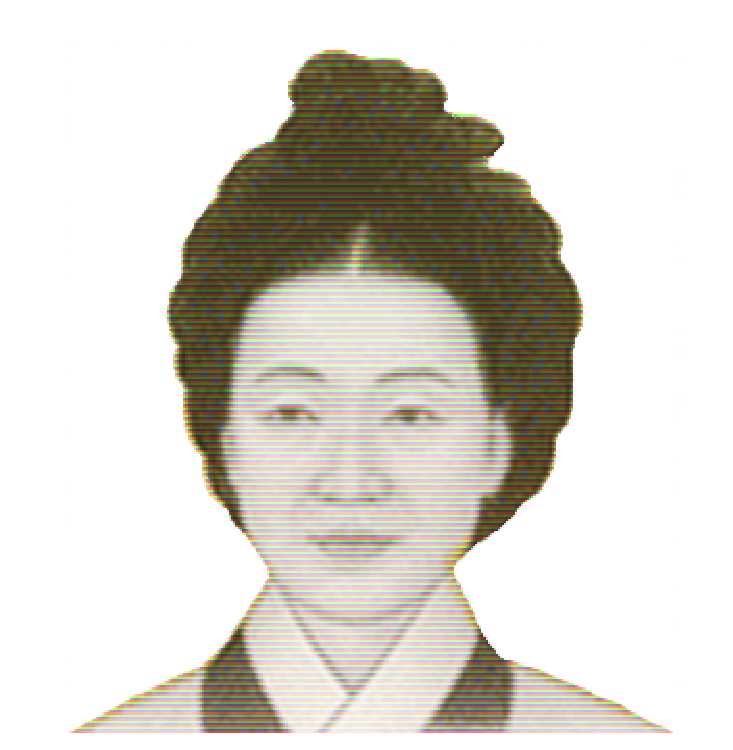
\includegraphics[height=8cm]{ssid-video}}
\psset{linestyle=none}
\pstextpath(0,0){%
\parametricplot[plotstyle=curve,plotpoints=1000]{0}{4100}{%
	t 1000 div dup t sin mul exch t cos mul}}{\texthan}
\end{pspicture}
\end{CJK}
\end{document}


* compilation

$ latex ssid && dvips ssid && ps2pdf ssid.ps
 

* original image source

http://en.wikipedia.org/wiki/File:50000_KRW_2009_ob.jpg

(processed by me and Gimp 2.6)


* text source

http://ko.wikipedia.org/wiki/신사임당
